\documentclass[]{article}
\usepackage[UTF8]{ctex}
\usepackage[a4paper,left=10mm,right=10mm,bottom=10mm,top=10mm]{geometry}
\usepackage{graphicx}
\usepackage{float}
\usepackage{amsmath,amsfonts,amssymb,amsthm}
\usepackage{array,color}
%opening
\title{计算机科学中的数学基础Exercise16}
\author{陈昱衡 521021910939}
\date{\today}

\begin{document}

\maketitle


\section*{Warmup1}
\begin{figure}[H]
    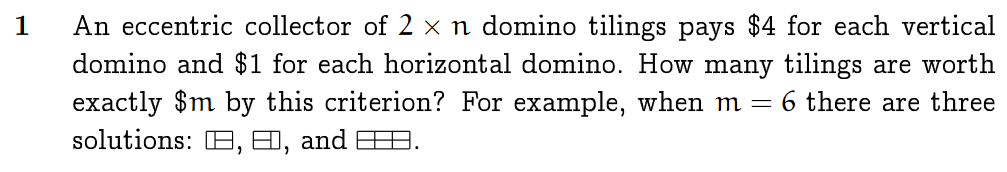
\includegraphics[scale = 0.6]{2023-04-06-10-50-30.png}
\end{figure}
我们可以仿照课本解决多米诺牌的思路,使用$z$替换水平放置的牌,使用$z^4$替换垂直放置的牌。\par 
同时,因为将两个叠放的多米诺牌看做一个整体,所以有
\begin{align}
    T &= 1 + z^4 T  + z^2 T\\
    T &= \frac{1}{1 - z^2 - z^4}
\end{align}
这个式子类似于斐波那契数,只不过将$z$变为$z^2$,故当$m$为奇数时,答案为零,当$m$为偶数时,
有
\begin{align}
    T_{\frac{m}{2}} &= F_{\frac{m}{2}+1}\\
\end{align}

\section*{Warmup2}
\begin{figure}[H]
    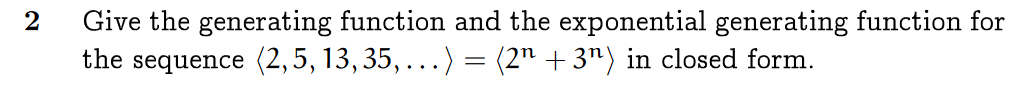
\includegraphics[scale = 0.6]{2023-04-06-10-51-32.png}
\end{figure}
由课本中表7-1中的结论,由已知的求和式和生成函数的线性性,有
\begin{align}
    2^n + 3^n &= \frac{1}{1-2z} + \frac{1}{1-3z}\\
    G(z) &= \frac{1}{1-2z} + \frac{1}{1-3z}\\
\end{align}
由指数生成函数及其封闭性的定义,等比数列$<1,p,p^2,\cdots>$的指数生成函数是:
\begin{align}
    \sum_{n \ge 0}\frac{p^n x^n}{n!} = e^{px}
\end{align}
再结合线性性,有
\begin{align}
    \hat{G(z)} &= e^{2z}+e^{3z}\\
\end{align}

\section*{Basics6}
\begin{figure}[H]
    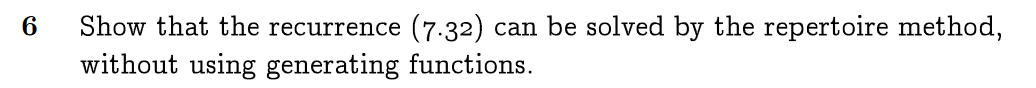
\includegraphics[scale = 0.6]{2023-04-06-10-51-49.png}
\end{figure}
使用成套方法,发现递归式中有三个系数,故令
\begin{align}
    g_0 &= \alpha\\
    g_1 &= \beta\\
    g_n &= g_{n-1}+g_{n-2} + (-1)^n \gamma\\
\end{align}
同时,$g_n$可表示为
\begin{equation}
    g_n = A(n) \alpha + B(n) \beta + C(n) \gamma
\end{equation}
观察这组式子,发现,使用$n$的多项式是无法配平的,因此,可以考虑$2^n$,$(-1)^n$,$(-1)^n n$;
将$g_n = 2^n$代入,有
\begin{align}
    \alpha  &= 1\\
    \beta &= 2\\
    \gamma &= 0\\
    2^n &= A(n) + 2B(n)\\
\end{align}
将$g_n = (-1)^n$代入,有
\begin{align}
    \alpha &= 1\\
    \beta &= -1 \\
    \gamma &= 0\\
    (-1)^n &= A(n)-B(n)\\
\end{align}
将$g_n = (-1)^n n$代入,有
\begin{align}
    \alpha &= 0\\
    \beta &= -1\\
    \gamma &= 3\\
    (-1)^n n &= -B(n) + 3C(n)\\
\end{align}
对上述三组关于$A(n),B(n),C(n)$的线性方程求解,有
\begin{align}
    A(n) &= \frac{2^n + 2 \times (-1)^n}{3}\\
    B(n) &= \frac{2^n - (-1)^n}{3}\\
    C(n) &= \frac{2^n + (3n-1)(-1)^n}{9}\\
\end{align}
因此,
\begin{align}
    g_n &= A(n) + B(n) +C(n)\\
    &=\frac{7}{9}2^n + (\frac{1}{3}n + \frac{2}{9})(-1)^n
\end{align}

\end{document}